\section{Definitions}
\label{sec:definitions}

One of the main reasons to introduce an \cstartb object-oriented framework \cendb is to enable sharing of knowledge between researchers, developers, and users. 
Therefore, it is important that the terms we use are clearly defined. 
When presenting our \cstartb object-oriented framework \cendb in \cref{sec:oo framework}, we will formalize the terms such that they can be used by software agents.
In this section, we will define the terms linguistically, thereby providing insight into the terms used in the next section.
We will first define the concept of a scenario in \cref{sec:scenario}. 
Next, we will define two important attributes of a scenario: events and activities, in \cref{sec:event,sec:activity}, respectively. 
Lastly, we will present the definition of a scenario category in \cref{sec:scenario category}.

In each of the \cref{sec:scenario,sec:event,sec:activity,sec:scenario category}, we start with background information. Next, we draw conclusions that lead to our proposed definition of the corresponding terms. After proposing a definition, we finish each section with remarks and implications of our proposed definition.



\subsection{Scenario}
\label{sec:scenario}

% Definition according to Go and Carroll
\textcite{go2004blind} describe a scenario within the field of system design. They define a scenario as ``a description that contains (1) actors, (2) background information on the actors and assumptions about their environment, (3) actors' goals or objectives, and (4) sequences of actions and events. Some applications may omit one of the elements or they may simply or implicitly express it. Although, in general, the elements of scenarios are the same in any field, the use of scenarios is quite different.'' 

% Definition according to Geyer et al.
\textcite{geyer2014} describe a scenario within the context of automated driving. They use the metaphor of a movie or a storybook for describing a scenario. \textcite{geyer2014} state that ``a scenario includes at least one situation within a scene including the scenery and dynamic elements. However, [a] scenario further includes the ongoing activity of one or both actors.'' For a further explanation of the terms situation, scene, and scenery, see \autocite{geyer2014}. 
%It is mentioned that the action of the driver and/or automation might be predefined. 
In \autocite{geyer2014}, the meaning of activity is not detailed.
%In an example of a so-called crossway scenario, they mention that the course of events might be different. For example, when a car keeps constant speed and then turns right, the scenario consists of one situation. The car might also first decelerate, accelerate and decelerate before turning right. In this case, the scenario consists of four situations.

% Definition according to Ulbrich et al.
\textcite{ulbrich2015} also define a scenario in the context of automated driving. They define a scenario as ``the temporal development between several scenes in a sequence of scenes. Every scenario starts with an initial scene. Actions \& events as well as goals \& values may be specified to characterize this temporal development in a scenario. Other than a scene, a scenario spans a certain amount of time.'' The authors of \autocite{ulbrich2015} state that actions and events link the different scenes. A further description of actions and events is not given in \autocite{ulbrich2015}

%\cstartb We consider scenes to correspond to a temporal snap shot of the entire scenario. Although a further description of actions and events is not given in \autocite{ulbrich2015}, we assume that they an event is marking a time point in the scenario. Therefore, each event  has a corresponding scene, and we can interpret this definition of scenario as meaning that
%a scenario has a start event (marking the scene at the start of the scenario), an end event which defines the time duration of the scenario, and a temporal sequence of events (corresponding to scenes) between the start event and the end event that mark the beginning/end of the ``actions''. 
%In particular, we understand that the existence of a scene is implied by the existence of an event, since the scene is just the temporal cross-section of the entire scenario at the time point of the event. \cendb

% Definition according to Elrofai et al.
Another definition of a scenario in the context of automated driving is given by \textcite{elrofai2016scenario}. They define a scenario as ``the combination of actions and maneuvers of the host vehicle in the passive [i.e., static] environment, and the ongoing activities and maneuvers of the immediate surrounding active [i.e., dynamic] environment for a certain period of time.'' They further mention that the duration of a scenario typically is in the order of seconds.

\cstartb
\textcite{catapult2018regulating} define a scenario as ``a description of a short interaction between an AV and other road users and/or road infrastructure''. 

In a concept paper on OpenSCENARIO 2.0 \autocite{OpenSCENARIO2}, a scenario is defined as ``a `description of the temporal development' of road users (actor entities) defined by their actions, where temporal activation (defining when) `is regulated by' conditional `triggers'. A scenario comprises both scenery and dynamic elements.'' \cendb

% What is missing in the definitions?
% 1. No difference between qualitative and quantitative. I.e., definitions are ambiguous.
% 2. There are undefined terms.
% 3. Definitions are not detailed enough to reflect into code.

%Although the aforementioned definitions of scenario \autocite{geyer2014, ulbrich2015, elrofai2016scenario} are in the context of automated driving, we require a more concrete definition. First, the aforementioned definitions do not specify the level of detail. 
%We experience much confusion where one group thinks a discussion is about a very specific scenario whereas another group thinks the same discussion is about a collection of scenarios that share some characteristics. 
%Secondly, the aforementioned definitions use undefined terms, such as ``action'' and ``event''. Thirdly, because scenarios are used to specify test cases for the assessment of AVs, a clear and unambiguous specification of these scenarios is important and the aforementioned definitions are not concrete enough to be directly reflected into a coding language.

% "Requirements"
Before providing the definition of the notion of scenario, characteristics of the notion of scenario based on literature are listed as follows:
\begin{enumerate}
	\item \textit{A scenario corresponds to a time interval:}
	The aforementioned definitions \autocite{go2004blind, geyer2014, ulbrich2015, elrofai2016scenario} state that a scenario corresponds to a time interval. \textcite{vannotten2003updated} call such a scenario a chain scenario (``like movies''), as opposed to a snapshot scenario, i.e., a scenario that describes the state at a time instant (``like photos''). %The duration of a scenario is in the order of seconds, as explicitly mentioned by \textcite{elrofai2016scenario}. Though the duration is not mentioned by \textcite{ulbrich2015}, the presented example is in the order of seconds. Furthermore, other scenarios regarding (automated) driving are also in the order of seconds, e.g., see \autocite{gietelink2006development, zofka2015datadrivetrafficscenarios, roesener2017comprehensive, karaduman2013interactivebehavior, hulshof2013autonomous, englund2016grand}.
	\cstartb Because a scenario corresponds to a time interval, in our object-oriented framework, a scenario is a subclass of the concept \emph{time interval}. \cendb

	% Scenarios consists of one or several events
	\item \textit{A scenario consists of \cstartb two or more \cendb events \autocite{vannotten2003updated, go2004blind, geyer2014, ulbrich2015, kahn1962}:}
	It can be helpful to develop scenarios using events \autocite{bishop2007scentechniques}. Thus, a scenario could be defined as a particular sequence of events or, as \textcite[p.~143]{kahn1962} writes, ``a scenario results from an attempt to describe in more or less detail some hypothetical sequence of events''. Furthermore, \textcite{geyer2014} and \textcite{ulbrich2015} use the notion of event for describing a scenario, although they do not provide a definition of the term \emph{event}. 
	\cstartb Because a scenario contains at least a start event and an end event, the minimum number of events is two. \cendb
	In \cref{sec:event}, we will elaborate on the notion of \emph{event}.

	% Semantically described
	\item \textit{Real-world traffic scenarios are quantitative scenarios:}
	Regarding the nature of the data, a scenario can be either qualitative or quantitative \autocite{vannotten2003updated}. Real-world traffic scenarios are quantitative scenarios, such that they are, e.g., suitable for simulation purposes. A scenario, however, can also be described qualitatively, such that it is readable and understandable for human experts. Providing a qualitative description of a quantitative scenario has become known as a story-and-simulation approach \autocite{alcamo2001scenarios}. 
	Note that several quantitative scenarios might have the same qualitative description; thus, a qualitative description of a scenario does not uniquely define a quantitative scenario. A qualitative description can be regarded as an abstraction of the quantitative scenario, see also \cref{sec:scenario category}.

	% Some relevance between events
	\item\textit{The time interval of a scenario contains all relevant events:}
	According to \textcite{geyer2014}, ``the end of a scenario is defined by the first irrelevant situation with respect to the scenario''. In a similar manner, we require that the time interval of a scenario should contain all relevant events. Note that `relevant' is subjective and, therefore, an event is considered to be relevant, if it is relevant to the ego vehicle.
	% Next to that, an event is regarded as irrelevant, if it is independent of the relevant events.

	% Description of environment
	\item\textit{A scenario includes the description of the environment:}
	A scenario should include the description of the static and dynamic environment.
	Although the description of the static environment is not a general prerequisite of a scenario, this is often included when speaking about traffic scenarios \autocite{geyer2014, ulbrich2015, elrofai2016scenario, ebner2011identifying, althoff2017CommonRoad}.
	%The static environment does not change during a scenario.
	The description of the dynamic environment includes a description of the type of actors and the goals and/or activities of the actors.
	\cstartb The static environment consists of all relevant physical things that do not have relevant changes with respect to the ego vehicle. The dynamic environment consists of all relevant physical things -- including actors -- that have changes that are relevant to the ego vehicle. For example, the road may be part of the static environment, but if the change in the road temperature is relevant to the ego vehicle, the road is part of the dynamic environment.\cendb
	
	\cstartb
	\item\textit{A scenario includes one ego vehicle \autocite{geyer2014, elrofai2016scenario}:}
	Because of the two previously mentioned characteristics, a scenario is required to include an ego vehicle.
	\cendb
	
	%Everything that changes during the time interval of a scenario is considered to be part of the dynamic environment. 
	
	% Goals (instead of activities)
	\item\textit{A scenario describes the goals or activities of the \cstartb actors:\cendb}
	\cstartb Either the activities, the goals, or a combination of activities and goals are required to determine the response of the actor. \cendb
	Note that this also holds for the ego vehicle since the ego vehicle is an actor.
	For describing a scenario in real-world data, it is not necessary to describe the goals and, therefore, \textcite{elrofai2016scenario} mention the activities of the \cstartb actors \cendb rather than the goals. When describing a scenario that an AV has to cope with, however, the ego vehicle's goals (i.e., its driving mission \autocite{geyer2014}) could be specified rather than its activities \autocite{ulbrich2015}. Note that if the activities of \cstartb an actor \cendb are described rather than its goals, an observer might not be able to determine whether the \cstartb actor \cendb has successfully responded to the scenario.
\end{enumerate}


% Definition
Hence, we define a scenario as follows:
\begin{definition}[Scenario]\label{def:scenario}
	A scenario is a quantitative description of the relevant characteristics of the ego vehicle, its activities and/or goals, its static environment, and its dynamic environment. In addition, a scenario contains all events that are relevant to the ego vehicle.
\end{definition}

% Describe difference from literature
% - quantitative --> to avoid ambiguous situation and to serve assessment
% - notion of scene not used. Scene follows from description, but is not explicitely used
%\Cref{def:scenario} deviates from existing definitions \autocite{geyer2014, ulbrich2015, elrofai2016scenario} in that it explicitly mentions that a scenario is quantitative. We use the term \emph{scenario class} to refer to the qualitative description, see \cref{sec:scenario class}.

\textcite{geyer2014} and \textcite{ulbrich2015} use the term \emph{scene} to define a scenario.
\cstartb Since we consider a scene to correspond to a temporal snapshot of the entire scenario, a scene can be obtained by taking a temporal cross-section of the entire scenario as described in \cref{def:scenario}. As such\cendb, the scenes do not have to be described explicitly.


%\Cref{fig:scenario} shows a schematic overview of the various components of a scenario. As shown in the second row of \cref{fig:scenario}, a scenario contains an ego vehicle, a dynamic environment, and a static environment. As an example, possible activities of the vehicle in front, which is part of the dynamic environment, are detailed by considering the state variables `heading' and `speed'. Note that a definition of the term activity is given in \cref{sec:activity}. The two rows of the activities show more generic descriptions and more detailed descriptions, respectively, of some possible activities.

%\begin{figure}
%	\centering
%	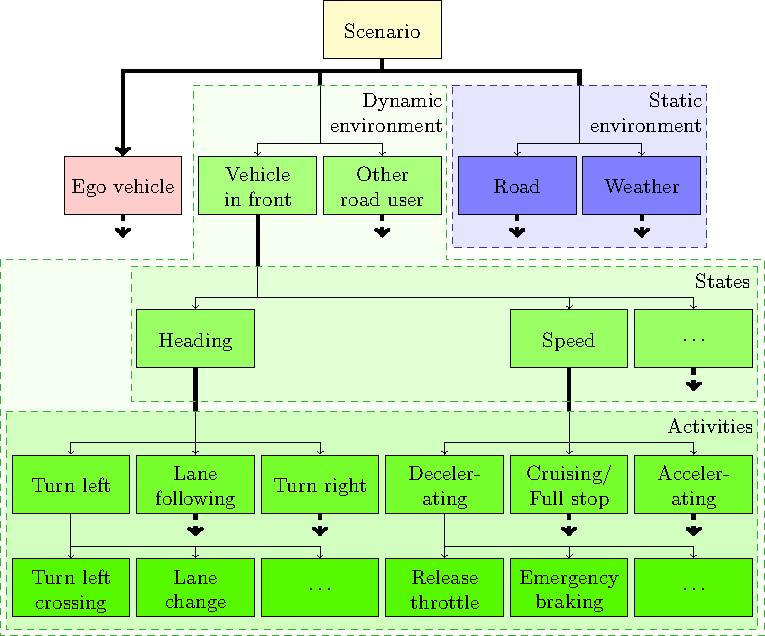
\includegraphics[width=0.5\linewidth]{figures/scenario.pdf}%
%	\caption{Schematic overview of a scenario. Note that the dynamic environment is not limited to the `vehicle in front', nor does it need to have the `vehicle in front'. Similarly, the static environment is not limited to `road', nor does it need to have `road'.}
%	\label{fig:scenario}
%\end{figure}


According to \cref{def:scenario}, a scenario describes, among others, the static environment. 
When it comes to applying this definition in an \cstartb object-oriented framework\cendb, it is possible that ``describing'' the static environment is done by simply providing a reference to a static environment. 
This also holds for the other parts of a scenario. 
A reference could be, for example, the full name of a file, a pointer pointing to a specific part of the computer memory, or an identifier that addresses a specific entry in a database.
The advantage of references is that these parts of the scenario can be exchanged across different scenarios, as these scenarios can use the same references. 
As an example, an OpenSCENARIO file allows to provide a reference to an OpenDRIVE file which describes a road network \autocite{dupuis2010opendrive}. As we will see in \cref{sec:oo framework}, in our proposed \cstartb framework\cendb, a scenario may contain references to a static environment, activities, actors, and events.
 


\subsection{Event}
\label{sec:event}

% Introduction of this section
As mentioned in \cref{def:scenario}, a scenario consists of events. 
%The notion of event is extensively used in literature \autocite{breu1997towards, pfeiffer2013concepts, branicky1998hybridcontrol, deschutter2000optimal, heemels2012eventcontrol}. In this section, a selected number of descriptions is presented. Next, a definition of event is given that suits our context.
% Literature review
The term event is used in many different fields, e.g.:
\begin{itemize}
	\item In computing \autocite{breu1997towards}, an event is an action or occurrence recognized by software. A common source of events are inputs by the software users. An event may trigger a state transition.
	%\item \textcite{kim1993supervenience}, a philosopher, writes: ``The term event ordinarily implies change''. \textcite{kim1993supervenience} states that an event is composed of three elements: objects, a property, and a time instant or a temporal interval. 
	
	\item In probability theory, an event is an outcome or a set of outcomes of an experiment \autocite{pfeiffer2013concepts}. For example, a thrown coin landing on its tail is an event.
	
	%\item ``In relativity, an event is any occurrence with which a definite time and a definite location are associated; it is an idealization in the sense that any actual event is bound to have a finite extent both in time and in space'' \autocite{sartori1996understanding}.
	
	\item In the field of hybrid systems theory, ``the continuous and discrete dynamics interact at `event' or `trigger' times when the continuous state [vector] hits certain prescribed sets in the continuous state space'' \autocite{branicky1998hybridcontrol}. ``A hybrid system can be in one of several modes, [...], and the system switches from one mode to another due to the occurrence of events'' \autocite{deschutter2000optimal}.
	
	\cstartb\item In ISO~15926, an ontology for long-term data integration, access, and exchange is specified in which an event is defined as ``a \emph{possible\_individual}\footnote{\cstartb ``An entity that exists in space and time'' \autocite{batres2007upper}.\cendb} with zero extent in time, which means that it occurs at an instant in time'' \autocite{batres2007upper}. \cendb
	
	\item In event-based control, a control action is computed when an event is triggered, as opposed to the more traditional approach where a control action is periodically computed \autocite{heemels2012eventcontrol}. In event-based control, the event is triggered at the moment at which the system (is about to) reach a certain threshold.
\end{itemize}

Before providing the definition of an event, the following is concluded about an event, based on aforementioned literature:

% It is a time instant
\begin{enumerate}
	\item\textit{An event corresponds to a time instant:}
	\cstart For the definition of event, we consider a hybrid-systems setting with a linear time model \autocite{alur1994theory}. Therefore, an event happens at some time instant.\cend
	
	% Event should mark transition of a state from one set to another - mention relation with hybrid control
	\item\textit{An event marks a mode transition or the moment a system reaches a threshold:} A mode transition may be \cstart induced \cend by either an abrupt change of an input signal, a change of a parameter, a change in the model, \cstart or an external cause. \cend It is also possible that the event marks the moment that a system reaches a threshold.
	
	%\item\textit{An event marks (a cause of) a mode transition}
	%Events mark the transition of mode, which is either a change of input, parameter or state. This is analogous to the way event is described in hybrid control \autocite{boel1999hybridcontrol}.
\end{enumerate}

% Give definition
Hence, we define an event as follows:
\begin{definition}[Event] \label{def:event}
	An event marks \cstart the moment a mode transition occurs or the moment a system reaches a specified threshold, where the former can be induced by both internal and external causes. \cend Before and after an event, the state vector \cstartb of one or more objects and/or activities in the scenario \cendb corresponds to two different modes.
\end{definition}

% Mention that there are basically two definitions. First definition more suitable for triggers for test cases. Second definition more suitable for observations and inputs.
\Cref{def:event} indicates that the moment of an event can be defined in two different ways: \cstart(1) by a mode transition or (2) by the system reaching a threshold. 
The first type of event, i.e., a mode transition can occur at the moment of a sudden driver input. Furthermore, an event might also be induced by an external cause, such as an environmental change. The second type of event, i.e., related to the system reaching a threshold, \cend is especially useful when describing test cases. For example, consider the ego vehicle approaching a pedestrian that is about to cross the road \autocite{seiniger2015test}. 
Here, the event marks the moment that the distance between the vehicle and pedestrian is less than $\distancecondition$ meters. 
At the moment of this event, the pedestrian starts to cross the road such that the vehicle impacts the pedestrian if it does not change its speed or direction \autocite{seiniger2015test}.
By using a variable threshold $\distancecondition$, the value is flexible and can be set differently to define multiple scenarios.

For the practical implementation of events, a set of conditions may be specified. In that case, the event occurs at the moment that the conditions are met. A condition could be on, e.g., the distance between the vehicle and pedestrian. In \autocite{openscenario}, an extensive list of possible conditions that can be used to define an event is given.


%This first type of event, i.e., at the moment at which the system reaches a threshold, is related to events in event-based control \autocite{heemels2012eventcontrol}, whereas the second type of event, i.e., at the moment at which a mode transition occurs, is related to events in hybrid theory \autocite{deschutter2000optimal}. 
%Especially when designing scenarios for testing purposes, an event of the first type might trigger an event of the second type. For example, consider a vehicle approaching a zebra crossing with a pedestrian (dummy) that is about to cross the road at the zebra crossing. When the distance between the vehicle and the zebra crossing becomes less than 20 meters (event of the first type), the pedestrian (dummy) starts crossing the road at the zebra crossing (event of the second type).


%The inter-event time interval, i.e., the time in between two events, corresponds to a certain activity. For example, when the longitudinal acceleration is negative during an inter-event time interval, the activity can be described by the label `braking'.
%Another example of an event is the time instant at which the head lights are turned on. In that case, the activities before and after the event can be described as `lights off' and `lights on', respectively.



\subsection{Activity}
\label{sec:activity}

As mentioned in \cref{def:scenario}, a scenario  includes  a description of the dynamic environment of the ego vehicle. To describe the dynamic environment, activities are used. Furthermore, a scenario may describe the activities of the ego vehicle. 
% [Following sentence removed, because too obvious]
% Therefore, next to events, activities can be seen as the building blocks of a scenario.

Both the terms activity \autocite{geyer2014, elrofai2018scenario, childress2015using, catapult2018musicc, sigsim2019glossary} and action \autocite{geyer2014, ulbrich2015, bagschik2017ontology} are used in the context of automated driving. Although, strictly speaking, the terms action and activity have a slightly different meaning, they are often used for the same purpose:
\begin{itemize}
	\item According to \textcite{ulbrich2015}, actions may be specified for characterizing the temporal development in a scenario.
	\item \textcite{elrofai2018scenario} consider an activity as a building block of the dynamic part of the scenario: ``An activity is a time evolution of state variables such as speed and heading to describe for instance a lane change, or a braking-to-standstill.''
	\item In a glossary for a scenario catalog development \autocite{catapult2018musicc}, an activity is defined as ``the state [vector] of an object over an interval of time. An activity starts with an event and ends with another event.''
%	\item According to the Cambridge Dictionary, an activity is defined as ``the doing of something, or something that you are doing, have done, or could do'' \autocite{cambridge2019activity}.
%	\item \textcite{caspersen1985physical} define physical activity ``as any bodily movement produced by skeletal muscles that result in energy expenditure''.
%	\item \textcite{bobick1997movement} simply states that an activity is a ``sequence of movements''. 
\end{itemize}


Before providing the definition of an activity, the following is concluded about an activity based on the aforementioned literature:

\begin{enumerate}
	% Time interval
	\item\textit{An activity corresponds to an inter-event time interval:}
	As opposed to an event, an activity spans over a certain time interval. Furthermore, the start and the end of an activity are marked by an event.
	\cstartb Because a scenario corresponds to a time interval, in our object-oriented framework, an activity is a subclass of the concept \emph{time interval}. \cendb
	
	% Describing the evolution of a state	
	\item\textit{An activity quantitatively describes the time evolution of a state variable:}
	Because activities are building blocks of a scenario and a scenario corresponds to a quantitative description, the activities themselves need to be quantitative as well. 
	Therefore, an activity describes the time evolution of one or more state variables, i.e., the trajectory of one or more state variables over an inter-event time interval that corresponds to the activity, where the term state variable is defined in \cref{sec:state variable}.
	
	% Performed by something (an actor?)
	\item\textit{An activity is performed by an actor:}
	An activity quantitatively describes the time evolution of one or more state variables and a state variable corresponds to an actor, e.g., the acceleration of a vehicle, and, therefore, an activity is performed by an actor. Note that the actor might be the ego vehicle. 
	%However, it might also be the case that a state does not correspond to an actor. For example, a state describing the weather conditions does not correspond to an actor, so if an activity describes changing weather conditions, the activity is not performed by an actor.
\end{enumerate}

Hence, we define an activity as follows:
\begin{definition}[Activity]
	\label{def:activity}
	An activity quantitatively describes the time evolution of one or more state variables of an actor between two events.
\end{definition}


% Remarks
% 1. Activity is very similar to mode, i.e., a model that describes the evolution of a state over time with parameters theta
% Skipped...

% 2. Activity vs. action
Note that \textcite{geyer2014, ulbrich2015} use the term \emph{action} and although they do not define this term, it seems to be related to our use of the term activity. Similarly, other authors \autocite{sigsim2019glossary, catapult2018musicc, elrofai2018scenario} use the term activity. Although the terms \emph{activity} and \emph{action} may seem very similar, there is a difference. As \textcite{bobick1997movement} points out, actions require an interpretive context --- ``a set of constraints on possible explanations for the observed motions.''
Considering our context of scenarios, i.e., the assessment of AVs, we are concerned with the occurrence of activities, because an AV needs to cope with them. The actual purpose of each of the activities is irrelevant concerning the assessment. Hence, we refrain from using the term \emph{action}.

% 3. Examples of activities
Examples of activities are accelerating, cruising, and decelerating. Here, the activities describe the longitudinal acceleration (or, e.g., speed). Activities describing the lateral position of a vehicle with respect to the center of the  corresponding lane  might, e.g., be labeled with ``driving straight'' or ``lane change''.




\subsection{Scenario category}
\label{sec:scenario category}

% Introduce term scenario category (i.e. qualitative description of scenario)
As proposed in \cref{def:scenario}, a scenario in the context of the performance assessment of an AV needs to be quantitative. 
However, in literature, the term scenario is also used to refer to a collection of scenarios, where this collection of scenarios is semantically described. For example, in \autocite{USDoT2007precrashscenarios}, a typology of pre-crash scenarios is proposed. Here, each of the pre-crash scenarios is an abstraction of many quantitative scenarios. Similar studies have been performed to describe scenarios that lead to highway accidents \autocite{adaptive2017d73}, car-cyclist accidents \autocite{opdencamp2014cats}, and car-pedestrian accidents \autocite{lenard2014typical}. In \autocite{catapult2017taxonomy}, a taxonomy of scenarios is proposed to qualitatively describe challenging scenarios for automated driving.

The aforementioned references \autocite{USDoT2007precrashscenarios, adaptive2017d73, opdencamp2014cats, lenard2014typical, catapult2017taxonomy} show that the term \emph{scenario} is also used to address qualitative descriptions. Since we defined a scenario as a quantitative description, we need to introduce a different term to address the qualitative description. We propose to use the term \emph{scenario category} to refer to the qualitative description of a scenario. A qualitative description can be regarded as an abstraction of a quantitative scenario, whereas a quantitative description can be regarded as a concretization of a qualitative description.

We thus define a scenario category as follows:
\begin{definition}[Scenario category] \label{def:scenario category}
	A scenario category is a qualitative description of the ego vehicle, its activities and/or goals, its static environment, and its dynamic environment.
\end{definition}

% What is the purpose of this?
% - Human interpretable
% - Group scenarios that are very similar --> Analysis is easier
% - Completeness
Introducing the concept of scenario categories brings the following benefits:
\begin{itemize}
	\item For a human, it is easier to interpret a qualitative description rather than a quantitative description.
	\item It enables to refer to a group of scenarios that have something in common. Therefore, it enables characterization of the type of scenarios, thus making discussing scenarios much easier.
	\item It allows for quantifying the completeness of a set of scenarios by separately quantifying the completeness of scenario categories and the completeness of scenarios in each category.
	This is easier because scenario categories are discrete by nature whereas scenarios are continuous. See \autocite{degelder2019completeness} for more details.
\end{itemize}

% Explain scenario category comprise scenarios
We describe the formal relation between a scenario and a scenario category with the verb ``to comprise'', denoted by $\comprises$. If a specific scenario category $\scenariocategory$ is an abstraction of a specific scenario $\scenario$, then we say that the specific scenario category $\scenariocategory$ comprises that specific $\scenario$, or simply $\scenariocategory \comprises \scenario$. 
This is illustrated in \cref{fig:venn diagram scenario category}, where $\scenarioa$, $\scenariob$, and $\scenarioc$ represent scenarios and $\scenariocategorya$, $\scenariocategoryb$, and $\scenariocategoryc$ represent scenario categories. 
A given scenario category can comprise multiple scenarios, e.g., $\scenariocategoryb \comprises \scenarioa$ and $\scenariocategoryb \comprises \scenariob$ in \cref{fig:venn diagram scenario category}. 
% Explain multiple scenario categories can comprise a scenario
Furthermore, multiple scenario categories can comprise a specific scenario.
For example, in \cref{fig:venn diagram scenario category}, we have $\scenariocategorya \comprises \scenariob$, $\scenariocategoryb \comprises \scenariob$, and $\scenariocategoryc \comprises \scenariob$. 

\setlength{\venncircle}{5em}
\begin{figure}[t]
	\centering
	\begin{tikzpicture}
	% Circles
	\fill[red, fill opacity=0.5] (-\venncircle/2, 0) circle (\venncircle);
	\fill[green, fill opacity=0.5] (\venncircle/2, 0) circle (\venncircle);
	\draw (-\venncircle/2, 0) circle (\venncircle);
	\draw (\venncircle/2, 0) circle (\venncircle);
	
	% Names of scenario classes
	\node[anchor=east](daylight) at (-5/4*\venncircle, \venncircle) {$\scenarioclassb$};
	\draw (daylight) -- ({(-sqrt(2)/2-1/2)*\venncircle}, {sqrt(2)/2*\venncircle});
	\node[anchor=west](rain) at (5/4*\venncircle, \venncircle) {$\scenarioclassc$};
	\draw (rain) -- ({(sqrt(2)/2+1/2)*\venncircle}, {sqrt(2)/2*\venncircle});
	\node[anchor=south](day and rain) at (-1/4*\venncircle, 8/7*\venncircle) {$\scenarioclassa$};
	\draw (day and rain) -- ({(1/2-sqrt(2)/2)*\venncircle}, {(sqrt(2)/2)*\venncircle});
	
	% Scenarios
	\node at (-0.1*\venncircle, -0.1*\venncircle) (scenariob){\textbullet};
	\node at (-\venncircle, 0.3*\venncircle) (scenarioa){\textbullet};
	\node at (\venncircle, 0.2*\venncircle) (scenarioc){\textbullet};
	\node[right of=scenarioa, node distance=1em]{$\scenarioa$};
	\node[right of=scenariob, node distance=1em]{$\scenariob$};
	\node[right of=scenarioc, node distance=1em]{$\scenarioc$};
	%\node[text width=\venncircle, align=center] at (-\venncircle, 0) {Scenarios without rain during daytime};
	%\node[text width=\venncircle, align=center] at (0, 0) {Scenarios with rain during daytime};
	%\node[text width=.9\venncircle, align=center] at (\venncircle, 0) {Scenarios with rain during nighttime};
\end{tikzpicture}

	\caption{The red and green circles correspond to the scenario categories $\scenariocategoryb$ and $\scenariocategoryc$, respectively. The overlap between the two circles corresponds to scenario category $\scenariocategorya$. The dots represent scenarios $\scenarioa$, $\scenariob$, and $\scenarioc$. %$\scenariocategoryb$ comprises $\scenarioa$ and $\scenariob$. $\scenariocategoryb$ and $\scenariocategoryc$ include $\scenariocategorya$.
	}
	\label{fig:venn diagram scenario category}
\end{figure}

% Explain scenario category can include scenario categories
The verb ``to include'' is used to describe the relation between two scenario categories. A scenario category $\scenariocategoryb$ is said to include a scenario category $\scenariocategorya$ if $\scenariocategoryb$ comprises all scenarios that are comprised in $\scenariocategorya$. In that case, we can write $\scenariocategoryb \includes \scenariocategorya$. Thus we have
\begin{equation} \label{eq:scenario category include}
	\scenariocategoryb \includes \scenariocategorya \text{ if } \scenariocategoryb \comprises \scenario\,\,\forall\,\, \{S: \scenariocategorya \comprises \scenario\}.
\end{equation}
%In \cref{fig:venn diagram scenario category}, scenario categories $\scenariocategoryb$ and $\scenariocategoryc$ include scenario category $\scenariocategorya$; thus $\scenariocategoryb \includes \scenariocategorya$ and $\scenariocategoryc \includes \scenariocategorya$.

% Figure is explained in last few paragraphs, but placed earlier as to appear at the right page of the paper.
\begin{figure}[t]
	\centering
	\begin{subfigure}{\linewidth}
		\centering
		\tree{Vehicle lateral activity}{Going straight; Changing lane, Left, Right; Turning, Left, Right; Swerving, Left, Right}
		\caption{Lateral activities of a vehicle.\vspace{1em}}
		\label{fig:tree vehicle lat act}
	\end{subfigure}
	\begin{subfigure}{\linewidth}
		\centering
		\tree{Vehicle longitudinal activity}{Reversing; Standing still; Driving forward, Braking, Cruising, Accelerating}
		\caption{Longitudinal activities of a vehicle.}
		\label{fig:tree vehicle long act}
	\end{subfigure}
	\caption{Tags for lateral and longitudinal activities of a vehicle. The lateral activity is relative to the lane in which the corresponding vehicle is driving.}
	\label{fig:tree vehicle activities}
\end{figure}

We propose to provide scenarios and scenario categories with additional information in the form of tags that describe the scenario in a qualitative manner.
Tags are often used when providing extra information on a piece of data \autocite{smith2007tagging}. A tag is a keyword or a term that helps describing an item. For example, items in a database can contain some tags that enable users to quickly obtain several items that share a certain characteristic described by a tag \autocite{craft2004tagging}. 
%Applications are very broad, e.g., from classification of audio data \autocite{kong2017joint} capturing musical characteristics from songs \autocite{ellis2011semantic} to tagging of Wikipedia pages \autocite{voss2006collaborative}.
The use of these tags brings several benefits:
\begin{itemize}
	\item The tags of a scenario can be helpful in determining which scenario categories do and do not comprise the scenario.
	%\item If a scenario category that only contains known tags is added to the database of scenario categories, it can easily be seen which scenarios the scenario category comprises by only inspecting the tags of the scenarios. Therefore, there is no need to define scenario categories a priori.
	\item It is easy to select scenarios from a scenario database or a scenario library by using tags or a combination of tags.
	\item As opposed to the proposed categorization of scenarios in \autocite{opdencamp2014cats, USDoT2007precrashscenarios, lenard2014typical, lara2019harmonized}, scenario categories do not need to be mutually exclusive.
\end{itemize}

There is a balance between having generic scenario categories --- and thus a wide variety among the scenarios belonging to the scenario category --- and having specific scenario categories without much variety among the scenarios in the scenario category. For some systems, one may be interested in very specific set of scenarios, while for another system one might be interested in a set of scenarios with a high variety. To accommodate this, tags can be structured in hierarchical trees \autocite{molloy2017dynamic}. The different layers of the trees can be regarded as different abstraction levels \autocite{Bonnin2014}. 

In \autocite{degelder2019scenariocategories}, several trees of tags are defined and \cref{fig:tree vehicle activities} shows two examples of trees of tags taken from \autocite{degelder2019scenariocategories}. These tags describe possible activities of a vehicle, i.e., the lateral motion control (via steering) and longitudinal motion control (via acceleration and deceleration) are reflected into tags. The tags may refer to the objective of an actor in case no activities are defined. For example, a test case in which the ego vehicle's objective is to make a left turn, the tags ``Turning'' and ``Left'' are applicable. Note that tags may be used not only to classify vehicle behavior, but also traffic and environment situations, e.g., ``cut-in'' or ``heavy rain''.

%Four different types of activities are identified regarding the lateral movement, see \cref{fig:tree vehicle lat act}. Here, it is assumed that ``lateral'' refers to the direction perpendicular to the lane the vehicle is driving in (e.g., according to the Road Coordinate System in \autocite{zofka2015datadrivetrafficscenarios}). Therefore, if the vehicle is driving on a curved road while staying more or less in its lane (lane-following), the tag ``Going straight'' is applicable. Apart from going straight, the vehicle might change lane, turn, or swerve to either the left or the right. 
 
%\Cref{fig:tree vehicle long act} shows tags regarding the longitudinal activity of a vehicle. 
